\documentclass[10pt]{article}
\usepackage[margin=0.9in]{geometry}
\usepackage{amsmath,amssymb,amsthm,graphicx,booktabs,hyperref,tikz,xcolor,seqsplit}
\usetikzlibrary{arrows.meta,positioning}
\newtheorem{theorem}{Theorem}
\newtheorem{lemma}{Lemma}
\newtheorem{proposition}{Proposition}
\newtheorem{corollary}{Corollary}
\newcommand{\norm}[1]{\left\lVert #1\right\rVert}
\newcommand{\ket}[1]{\lvert #1\rangle}
\newcommand{\bra}[1]{\langle #1\rvert}
\newcommand{\eps}{\varepsilon}
\newcommand{\tr}{\mathsf T}
\newcommand{\Tr}{\operatorname{Tr}}
\newcommand{\E}{\mathcal E}
\graphicspath{{figures/}}
\begin{document}
\title{Supplementary Derivations and Timing Projection for Polynomial Quantum Recurrent Channels}
\author{Vahid Tavakkoli, Kabeh Mohsenzadegan, and Kyandoghere Kyamakya}
\date{October 2026}
\maketitle
\noindent This supplement preserves derivations and historical-topology projections
relocated from the 21-page main manuscript. No additional quantum hardware
measurements are claimed.\par
\appendix


\section{Classical Matrix-Flow Motivation and Its Limits}\label{sec:classicalmotivation}
This appendix preserves the classical antecedent without treating a matrix ODE as a quantum channel or attributing its classical inverse-matrix state to the quantum data register.
The 2019 recurrent model includes, in its notation, a polynomial sum in $M^{\tr}M$ and a matrix-derivative compensation term \cite[Eq. (24)]{r4}. With renamed gain $\eta>0$ and degree $s$, its form is
\begin{equation}\label{eq:2019}
M\dot X=\eta\sum_{j=0}^{s}(M^{\tr}M)^j(I-MX)-\dot M X.
\end{equation}
The equation investigated here is a separate motivating variant, not a quotation of that model. Set $S=MM^{\tr}$, $B=I-\mu S$, $P=(I+\alpha S)^m$, where $\alpha>0$, $m\ge0$ and $0<\mu<\norm M_2^{-2}$. Consider
\begin{equation}\label{eq:classical}
M\dot X B=P(I-MX).
\end{equation}
\begin{theorem}[Constant-matrix stability]\label{thm:classical}
For a constant nonsingular $M$, \eqref{eq:classical} has a unique velocity for each $X$, and $E=I-MX$ satisfies $\dot E=-PEB^{-1}$. If $\sigma_{\min}$ is the smallest singular value, then
\begin{equation}\label{eq:classicalrate}
\norm{E(t)}_F\le e^{-\nu t}\norm{E(0)}_F,\qquad
\nu=\frac{(1+\alpha\sigma_{\min}^2)^m}{1-\mu\sigma_{\min}^2}>0.
\end{equation}
\end{theorem}
\begin{proof}
The stated interval makes $B$ positive definite, and $M$ is invertible. Diagonalize $S=Q\operatorname{diag}(\sigma_i^2)Q^{\tr}$. In $\widetilde E=Q^{\tr}EQ$, each entry obeys
\[
\dot{\widetilde E}_{ij}=-\frac{(1+\alpha\sigma_i^2)^m}{1-\mu\sigma_j^2}\widetilde E_{ij}.
\]
The smallest rate is $\nu$; squaring and summing the scalar solutions proves the result. Since $X-M^{-1}=-M^{-1}E$, inversion follows.
\end{proof}
An unscaled derivative factor $I-MM^{\tr}$ is singular whenever a singular value equals one. If a singular value exceeds one, the factor can be indefinite, and the same scalar modes can grow. The derivative-side factor therefore requires an explicit admissibility condition. Increasing $m$ boosts the continuous rate but also increases stiffness and polynomial evaluation cost. Small singular values and high condition numbers remain limiting after practical scaling.

Equation \eqref{eq:classical} is implicit: evaluating $\dot X$ generally requires solving with both $M$ and $B$. Writing it as a differential equation does not make it inverse-free. An explicit Euler discretization also requires its own step-size stability analysis. Neither the continuous rate nor its units can be transferred to a discrete quantum channel by analogy.

\subsection{Changing matrices and compensation}
For $M(t)$ and the uncompensated \eqref{eq:classical},
\begin{equation}\label{eq:forcing}
\dot E=-PEB^{-1}-\dot M X.
\end{equation}
The compensation needed to recover $\dot E=-PEB^{-1}$ is
\begin{equation}\label{eq:compensation}
M\dot X B=PE-\dot M X B.
\end{equation}
For uniformly positive $B(t)$, the Frobenius energy obeys $\tfrac12\frac{d}{dt}\norm E_F^2\le-\nu(t)\norm E_F^2$ with the instantaneous rate in \eqref{eq:classicalrate}. This classical argument does not assume that matrices at distinct times commute. Without compensation, a bounded forcing term produces a tracking floor; near singularity the required velocity can be large. The quantum recurrent construction in the main text addresses a moving fixed state through a channel tracking inequality rather than implementing \eqref{eq:compensation} as an oracle.


\section{Auxiliary Snapshot Chebyshev--LCU Inverse Action}\label{sec:snapshot}
This appendix documents a separate one-shot reciprocal construction under dense spectral preprocessing. It serves as an auxiliary reference and is not the proposed polynomial recurrent algorithm.
For this section only, denote the positive upper singular bound by $b$ and the right-hand side by $b_0$. A reusable circuit has success block $X_d/\alpha_d$, where $X_d=Vp_d(\Sigma)U^{\tr}$; its action is independent of which valid input is supplied. The following established construction and certificate are retained to distinguish a snapshot inverse operator from the recurrent solution-state channel.

% Begin lcu.tex
For $a<b$, define
\begin{equation}\label{eq:param}
 \begin{aligned}
 c&=\frac{a+b}{2},\qquad h=\frac{b-a}{2},\\
 t&=\frac{\sigma-c}{h},\qquad
 r=\frac{\sqrt b-\sqrt a}{\sqrt b+\sqrt a}\in(0,1).
 \end{aligned}
\end{equation}
With $T_k(\cos\theta)=\cos(k\theta)$, use the degree-$d$ polynomial
\begin{equation}\label{eq:poly}
 p_d(\sigma)=\frac{1}{\sqrt{ab}}\left[1+2\sum_{k=1}^{d}(-r)^kT_k(t)\right].
\end{equation}
This is a truncated reciprocal series, not a claim that this polynomial is the optimal minimax approximation under every cost model.

\begin{lemma}[Uniform truncation]\label{lem:tail}
For $\sigma\in[a,b]$,
\begin{equation}\label{eq:tail}
 |p_d(\sigma)-\sigma^{-1}|\le E_d
 :=\frac{2}{\sqrt{ab}}\frac{r^{d+1}}{1-r}.
\end{equation}
\end{lemma}
\begin{proof}
The Poisson-kernel identity gives
\[
 1+2\sum_{k\ge1}(-r)^k\cos(k\theta)
 =\frac{1-r^2}{1+2r\cos\theta+r^2}
 =\frac{\sqrt{ab}}{c+h\cos\theta}.
\]
The omitted terms are bounded using $|T_k(t)|\le1$ and the geometric-series tail.
\end{proof}
Define
\begin{equation}\label{eq:delta}
 X_d=Vp_d(\Sigma)U^{\tr},\qquad
 \delta_d=bE_d=\frac{2\sqrt\kappa\,r^{d+1}}{1-r}.
\end{equation}

\begin{theorem}[Two-sided inverse-action certificate]\label{thm:op}
Under the singular-value decomposition,
\begin{align}
 \norm{MX_d-I}_2,\ \norm{X_dM-I}_2&\le\delta_d,\label{eq:residual}\\
 \norm{X_d-M^{-1}}_2&\le E_d.\label{eq:inverse}
\end{align}
For $x=M^{-1}b_0$ and $x_d=X_db_0$, both the relative residual $\norm{Mx_d-b_0}_2/\norm{b_0}_2$ and the relative solution error $\norm{x_d-x}_2/\norm{x}_2$ are at most $\delta_d$. If $\delta_d<1$, the normalized-state distance is at most $2\delta_d$.
\end{theorem}
\begin{proof}
$MX_d$ and $X_dM$ are orthogonal similarities of $\operatorname{diag}(\sigma_jp_d(\sigma_j))$, proving the residual bounds. Equation~\eqref{eq:inverse} follows directly from the singular bases. More generally,
$x_d-x=(X_dM-I)x$, which proves the relative solution bound without a further condition-number factor. For nonzero $u,v$,
\begin{equation}\label{eq:normalize}
 \norm{\frac{u}{\norm u_2}-\frac{v}{\norm v_2}}_2
 \le\frac{2\norm{u-v}_2}{\norm v_2}.
\end{equation}
Apply \eqref{eq:normalize} with $u=x_d,v=x$; $\delta_d<1$ ensures $x_d\ne0$.
\end{proof}

For $0<\eps<1$, a sufficient nonnegative degree is
\begin{equation}\label{eq:degree}
 d\ge \max\left\{0,
 \left\lceil\frac{\log[2\sqrt\kappa/((1-r)\eps)]}{-\log r}\right\rceil-1\right\}.
\end{equation}
Thus $d=O(\sqrt\kappa[\log\kappa+\log(1/\eps)])$ for large $\kappa$, conditional on the given spectral representation. If $a=b$, the constant polynomial $p_0=1/a$ is exact. At every fixed nonsingular finite instance, the degree required by \eqref{eq:degree} is finite. The result is not uniform as the gap tends to zero.

\noindent\textbf{Why singular values rather than normal equations?}
Indefinite and nonsymmetric matrices are covered through $U$ and $V$, while the reciprocal approximation acts on positive singular values. Forming normal equations would square the condition number; the stated construction does not approximate the inverse of $MM^{\tr}$ as an intermediate solver. This is a modeling choice, not a new singular-value factorization theorem. Repeated singular values also cause no ambiguity in the realized inverse action: admissible basis changes within a degenerate singular subspace leave $Vp_d(\Sigma)U^{\tr}$ unchanged.

\subsection{Coherent walk, selector, and reuse}\label{sec:circuit}
For singular coordinate $j$, set $\theta_j=\arccos[(\sigma_j-c)/h]$ and introduce the flag rotation
\begin{equation}\label{eq:rotation}
 R_j=\begin{bmatrix}\cos\theta_j&\sin\theta_j\\-\sin\theta_j&\cos\theta_j\end{bmatrix},
 \qquad \bra0 R_j^k\ket0=T_k(t_j).
\end{equation}
Let $W$ be the corresponding multiplexed walk on the flag/data register. With $c_0=1/\sqrt{ab}$ and $c_k=2(-r)^k/\sqrt{ab}$ for $k>0$, define
\begin{equation}\label{eq:alpha}
 \alpha_d=\sum_{k=0}^d|c_k|
 =\frac{1}{\sqrt{ab}}\left[1+\frac{2r(1-r^d)}{1-r}\right].
\end{equation}
PREP maps $\ket{0^s}$ to $\ket w=\sum_{k=0}^d\sqrt{|c_k|/\alpha_d}\ket k$. SELECT applies $\operatorname{sgn}(c_k)W^k$ on branch $k$. The alternating sign is implemented by a $Z$ on the selector's least significant bit. Branches above $d$ have zero preparation amplitude and receive a unitary extension.

Projecting PREP$^{\dagger}$ onto zero yields
\begin{equation}\label{eq:lcu}
 \bra{0^s,0}{\rm PREP}^{\dagger}{\rm SELECT}{\rm PREP}\ket{0^s,0}
 =p_d(\Sigma)/\alpha_d.
\end{equation}
Prepending $U^{\tr}$ and appending $V$ realizes the stated inverse-action block. Binary selector bits control commuting powers $R_j^{2^\ell}$, implemented by angle scaling of known multiplexed rotations. There are $s$ such power gadgets, but each gadget has a data-dependent synthesis cost; counting gadgets alone does not give the number of physical gates. Figure~2 of the main manuscript shows the operator structure.

\begin{figure}[!tbp]\centering
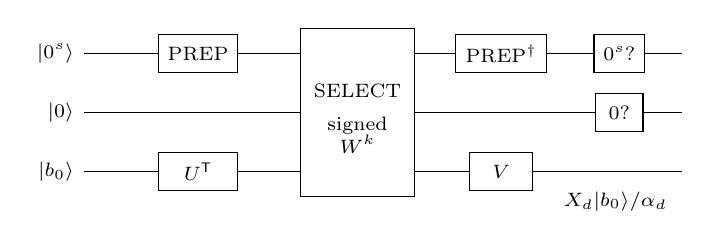
\begin{tikzpicture}[x=1cm,y=1cm,>=Latex,font=\scriptsize]
\draw (0,1.5)--(7.6,1.5);\draw (0,.75)--(7.6,.75);\draw (0,0)--(7.6,0);
\node[left] at (0,1.5) {$\ket{0^s}$};\node[left] at (0,.75) {$\ket0$};\node[left] at (0,0) {$\ket{b_0}$};
\node[draw,fill=white,minimum width=1cm,minimum height=.48cm] at (1.45,1.5) {PREP};
\node[draw,fill=white,minimum width=1cm,minimum height=.48cm] at (1.45,0) {$U^{\tr}$};
\draw[fill=white] (2.75,-.32) rectangle (4.2,1.82);
\node at (3.475,1.02) {SELECT};\node[align=center] at (3.475,.46) {signed\\$W^k$};
\node[draw,fill=white,minimum width=1.15cm,minimum height=.48cm] at (5.3,1.5) {PREP$^\dagger$};
\node[draw,fill=white,minimum width=.8cm,minimum height=.48cm] at (5.3,0) {$V$};
\node[draw,fill=white,minimum width=.6cm,minimum height=.48cm] at (6.8,1.5) {$0^s$?};
\node[draw,fill=white,minimum width=.6cm,minimum height=.48cm] at (6.8,.75) {$0$?};
\node[below] at (6.75,-.13) {$X_d\ket{b_0}/\alpha_d$};
\end{tikzpicture}
\caption{Unfused operator structure. PREP acts only on the selector, while $U^{\tr}$ and $V$ act on the data register. Both ancilla registers are heralded at zero. Input preparation and any subsequent reference verifier are separate operations.}
\label{fig:circuit}
\end{figure}

\begin{proposition}[Acceptance and magnitude]\label{prop:success}
For $a<b$, $\alpha_d\le1/a$. A normalized valid input succeeds with
\begin{equation}\label{eq:success}
 p_{\rm succ}=\frac{\norm{X_d\ket{b_0}}_2^2}{\alpha_d^2}
 \ge\frac{(1-\delta_d)^2}{\alpha_d^2 b^2}
 \ge\frac{(1-\delta_d)^2}{\kappa^2},
\end{equation}
provided $\delta_d<1$. Moreover, $\norm{X_db_0}_2=\alpha_d\norm{b_0}_2\sqrt{p_{\rm succ}}$ in the ideal model.
\end{proposition}
\begin{proof}
The infinite absolute coefficient sum is $1/a$, hence so is an upper bound on its truncation. The smallest singular value of $X_d$ is at least $(1-\delta_d)/b$ by \eqref{eq:residual}. The probability and magnitude identities follow from the successful block norm.
\end{proof}

Independent repetition has mean cost $1/p_{\rm succ}$ per accepted output; amplitude amplification is not implemented. For $\kappa=1000$, the lower bound is of order $10^{-6}$; a small register does not imply a modest repetition cost.


% End lcu.tex


\subsection{Temporal certificate for a held inverse operator}
Let $\widehat M=M_t+\Delta_t$, $\norm{\Delta_t}\le\eta$, and let $X$ approximate $\widehat M^{-1}$ with $\norm{\widehat M X-I}\le\delta<1$. At a later time $s$, suppose $\norm{M_s-M_t}\le L|s-t|$ and the implemented inverse-action block is $X+J$, $\norm J\le\xi$. Then
\begin{equation}\label{eq:held}
\norm{M_s(X+J)-I}\le\delta+(\eta+L|s-t|)\norm X+\norm{M_s}\xi.
\end{equation}
This follows by adding and subtracting $\widehat M X$. It is a sufficient operator-residual budget, not a statement that a snapshot-compiled circuit updates itself. If the right side exceeds the required tolerance, refresh or improved compilation is needed. A refresh is classical compilation plus a new quantum operation, and its latency belongs in any future real-time benchmark.



\subsection{Historical-topology timing projection}
To test routing sensitivity, we route the eight complete cost circuits and their three measurement settings on the public seven-qubit Jakarta topology. Table~\ref{tab:chebrouted} uses the pinned IBM Runtime snapshot dated 27 May 2024, not a current device calibration \cite{jakarta}. Edge-specific CX durations, qubit-specific readout durations and actual routed circuits are retained. Reset duration remains an assumed $1\,\mu$s; compilation reuse is 1000. The projected time charges the same conservative ideal confidence workload as Table~the main-manuscript readout table.
\begin{table}[!tbp]\centering\small\caption{Historical-topology projection. CX counts refer to the reference-population measurement setting; every setting has its own archived circuit and latency. Times exclude calibration noise and do not certify achievable hardware accuracy.}\label{tab:chebrouted}
% Begin tables/cheb-routed.tex
\begin{tabular}{rlrr}\toprule
$\kappa$ & Method & Routed CX & Time (s)\\\midrule
2 & Original & 6952 & 14699\\
2 & Power 4 & 1590 & 3447.4\\
2 & Power 16 & 1243 & 2659.5\\
2 & Chebyshev QSP & 6339 & 16040\\
10 & Original & 158738 & 8.5139e+06\\
10 & Power 4 & 31908 & 1.7124e+06\\
10 & Power 16 & 9694 & 5.2467e+05\\
10 & Chebyshev QSP & 17983 & 1.1715e+06\\
\bottomrule\end{tabular}

% End tables/cheb-routed.tex
\end{table}
At condition 2, the original-to-QSP projected-time ratio is 0.916. At condition 10, the original-to-QSP projected-time ratio is 7.27. A gate-count reduction can therefore coexist with a larger projected latency. These calculations measure a conditional implementation workload, not a hardware speedup. Snapshot gate and readout errors are not applied to the confidence calculation. Without a noisy-accuracy and bias analysis, a finite projected time must not be interpreted as an achievable physical time-to-solution. The public snapshot files, upstream source revision, routed QPY files and hash-linked audit are included in the reproduction archive.






\section{Validation-Selected Total-Cost Frontier: Reproduction and Cost Model}
\label{sec:costfrontierappendix}
This additional experiment evaluates the research question: under which drift,
logical-noise, and destructive-measurement conditions does a resident signed
Chebyshev quantum channel require less \emph{total resource-equivalent work}
than freshly preparing the solution state? The answer depends on the required
accuracy and readout schedule, rather than on recurrence iteration counts alone.

\subsection{Cost inequality and independent quantum copies}
Let $\mathcal{T}$ index the observed snapshots, $S=(N+1)H$ be the independent
measurement copies per checkpoint, and $d_j,K_j$ be method $j$'s selected
degree and recurrent macro count. A resident copy read at time $t$ must start
from a newly prepared reference state and propagate through all $t+1$
different inputs. It cannot be cloned after an earlier destructive readout.
Under the deliberately optimistic assumption that compilation is amortized
once per distinct input snapshot, the method costs are
\begin{align}
C_{\mathrm{res}}&=S(2d_rK_rw_q+K_rw_R)
\sum_{t\in\mathcal{T}}(t+1)
+S|\mathcal{T}|(w_P+w_M)
+(\max\mathcal{T}+1)w_C,\label{eq:cost_res_supp}\\
C_{\mathrm{fresh}}&=S(2d_fK_fw_q+K_fw_R)
|\mathcal{T}|+
S|\mathcal{T}|(w_P+w_M)
+|\mathcal{T}|w_C.\label{eq:cost_fresh_supp}
\end{align}
Here $w_q,w_R,w_P,w_M,w_C$ weight the oracle call, per-macro reset, a newly
prepared reference state, a destructive measurement execution, and distinct
input compilation. In this specific model, residence is strictly cheaper
among \emph{equally accuracy-qualified} policies if and only if
\begin{align}
S(2d_rK_rw_q+K_rw_R)\sum_{t\in\mathcal{T}}(t+1)
+(\max\mathcal{T}+1)w_C\;\;<\notag\\
S(2d_fK_fw_q+K_fw_R)|\mathcal{T}|+|\mathcal{T}|w_C.\label{eq:cost_break_even_supp}
\end{align}
If degrees and counts match, $d_r=d_f$ and $K_r=K_f$, and all weights are
nonnegative, the left-hand side is at least as large as the right-hand side.
A genuine positive break-even needs smaller charged resident updates,
a less destructive task, or a separately justified physical saving.
For direct postselection with success probability $p_t$, the expected
primitive calls per accepted copy are $2d/p_t$, and expected reference
preparations are $1/p_t$. The reported direct-control costs include these
retries and are not confused with unconditional channel updates.

\subsection{Parameter selection, accuracy, and scope}
The full fixed grid has three input families, five angular drift controls,
six logical per-oracle depolarization rates and four readout intervals,
for 360 scenarios. Both matrix dimension $N=2$ and condition $\kappa=10$
are held fixed; a 12-snapshot path is used. The maximum is 256 primitive
oracle calls per snapshot. Candidate degrees are derived from nominal
Chebyshev suppression targets $\{0.3,0.1,0.03\}$; macro counts are chosen
from $\{1,2,3,4,6,8\}$ subject to the budget.
Resident and fresh policies are selected \emph{only} on seeds 23 and 29.
Their selected degree and count remain fixed on disjoint held-out seeds
41 and 43. Eligibility requires at least 90\% of the observed checkpoints
to satisfy conditional infidelity at most 0.01 and relative residual at
most 0.05. This threshold differs from the strict $10^{-3}$ matched study,
which is reported independently and must not be pooled with this study.
Logical noise is not hardware-calibrated. Exact density-matrix scoring is
used; $H=16$ represents \emph{charged} shots per setting and does not
constitute actual finite-shot noisy readout or a confidence interval.

Illustrative resource-equivalent weights are
$(w_q,w_R,w_P,w_M,w_C)=(1,2,5,0.1,10)$. They are not measured
physical gate times. Classical input construction, physical reset latency,
device readout error and time to compile changing native circuits are not
experimentally calibrated. In particular, the separate compiled-native
small-instance QSP study is not automatically transferred to these logical
channel trajectories.

\begin{table}[!htbp]\centering\small
\caption{Held-out recurrent outcomes by logical per-oracle noise in the
360-scenario cost frontier. Column order: fresh cheaper when both qualify
(F), resident-only feasible (R), fresh-only feasible (F-only), and neither
recurrent method feasible (None). Resident is never lower-cost when both qualify.}
\label{tab:costfrontiernoise}
\begin{tabular}{lrrrr}\toprule
Noise & F & R & F-only & None\\\midrule
$0$ & 37 & 19 & 1 & 3\\
$10^{-6}$ & 37 & 19 & 1 & 3\\
$10^{-5}$ & 37 & 17 & 1 & 5\\
$2\cdot10^{-5}$ & 37 & 17 & 1 & 5\\
$5\cdot10^{-5}$ & 36 & 2 & 0 & 22\\
$10^{-4}$ & 0 & 0 & 0 & 60\\\bottomrule
\end{tabular}
\end{table}

\begin{table}[!htbp]\centering\small
\caption{Held-out recurrent outcomes by input angular-drift control
(rad/snapshot), with the same columns as Table~\ref{tab:costfrontiernoise}.
Angular input controls are not necessarily equal to target-projector drift.}
\label{tab:costfrontierdrift}
\begin{tabular}{lrrrr}\toprule
Drift & F & R & F-only & None\\\midrule
$0$ & 60 & 0 & 0 & 12\\
$0.01$ & 60 & 0 & 0 & 12\\
$0.05$ & 40 & 11 & 0 & 21\\
$0.2$ & 0 & 42 & 0 & 30\\
$0.6$ & 24 & 21 & 4 & 23\\\bottomrule
\end{tabular}
\end{table}

Among the 184 jointly qualified resident/fresh cases, the median ratio
$C_{\mathrm{res}}/C_{\mathrm{fresh}}$ is 3.122 (minimum 2.190, maximum
8.569). Resident is the only accuracy-qualified recurrent method in 74
additional cases, but is not therefore demonstrated to have lower cost
than an \emph{equally accurate} fresh option. Direct postselection is
the lowest-cost qualified method in 216 scenarios, fresh recurrence in 36,
resident recurrence in 20, and no method qualifies in 88.
The latter classification differs from the 98 scenarios where
neither \emph{recurrent} method qualifies because direct filtering
still qualifies in ten. These are deterministic conditional counts
on two test seeds, not confidence statements about real deployments.

\noindent\textbf{Integrity and source-pinned reproduction.}
The uploaded full-grid archive \texttt{total-cost.zip} has SHA-256
\texttt{\seqsplit{3fcc13ac7602181fb140d8e8d462d1647974799df3eabcbca0c902996f254b43}},
and its internal \texttt{MANIFEST.json} checksums match. An independent
\emph{full}, source-pinned GitHub Actions re-execution with Python 3.12.15
at commit \texttt{\seqsplit{f8917598c4cd4151cdb88f42acdd910d420257c4}}
(\url{https://github.com/vtavakkoli/QCeNN-MI/actions/runs/40682550700})
reproduces every one of the 360 scenario classifications, validation-selected
degree/update policies, and cheapest qualifying comparator. The compiled
\path{qcenn_mi.total_cost_phase_diagram} source SHA-256 is
\texttt{\seqsplit{d599ccc6ba04c78e885a8e49db3fe5b9e14616e772b0519afe1a7278804f90a2}}.
Individual floats may vary across numerical environments by at most
$1.5\times10^{-8}$ in these two compared results; raw JSON/CSV files are
therefore not byte-identical, but no accuracy decision or cost winner changes.
The original user-uploaded ZIP itself lacks a source-commit declaration,
and neither reproduced report is hardware timing or finite-shot output
certification.


\begin{thebibliography}{2}
\bibitem{r4} V. Tavakkoli, J. C. Chedjou, and K. Kyamakya,
``A novel recurrent neural network-based ultra-fast, robust, and scalable solver
for inverting a time-varying matrix,'' \emph{Sensors}, 19(18), 4002, 2019,
\url{https://doi.org/10.3390/s19184002}.
\bibitem{jakarta} IBM Quantum, ``Public Jakarta backend configuration and
properties,'' Qiskit IBM Runtime repository, snapshot May 27, 2024,
\url{https://github.com/Qiskit/qiskit-ibm-runtime/tree/main/qiskit_ibm_runtime/fake_provider/backends/jakarta}.
\end{thebibliography}
\end{document}
